%File: anonymous-submission-latex-2024.tex
\documentclass[letterpaper]{article} % DO NOT CHANGE THIS
\usepackage{aaai24}  % DO NOT CHANGE THIS
\usepackage{times}  % DO NOT CHANGE THIS
\usepackage{helvet}  % DO NOT CHANGE THIS
\usepackage{courier}  % DO NOT CHANGE THIS
\usepackage[hyphens]{url}  % DO NOT CHANGE THIS
\usepackage{graphicx} % DO NOT CHANGE THIS
\urlstyle{rm} % DO NOT CHANGE THIS
\def\UrlFont{\rm}  % DO NOT CHANGE THIS
\usepackage{natbib}  % DO NOT CHANGE THIS AND DO NOT ADD ANY OPTIONS TO IT
\usepackage[font=footnotesize,labelfont=bf]{caption} % DO NOT CHANGE THIS AND DO NOT ADD ANY OPTIONS TO IT
\frenchspacing  % DO NOT CHANGE THIS
\setlength{\pdfpagewidth}{8.5in} % DO NOT CHANGE THIS
\setlength{\pdfpageheight}{11in} % DO NOT CHANGE THIS
%
% These are recommended to typeset algorithms but not required. See the subsubsection on algorithms. Remove them if you don't have algorithms in your paper.
\usepackage{algorithm}
\usepackage{algorithmic}

%
% These are are recommended to typeset listings but not required. See the subsubsection on listing. Remove this block if you don't have listings in your paper.
\usepackage{newfloat}
\usepackage{listings}
\DeclareCaptionStyle{ruled}{labelfont=normalfont,labelsep=colon,strut=off} % DO NOT CHANGE THIS
\lstset{%
	basicstyle={\footnotesize\ttfamily},% footnotesize acceptable for monospace
	numbers=left,numberstyle=\footnotesize,xleftmargin=2em,% show line numbers, remove this entire line if you don't want the numbers.
	aboveskip=0pt,belowskip=0pt,%
	showstringspaces=false,tabsize=2,breaklines=true}
\floatstyle{ruled}
\newfloat{listing}{tb}{lst}{}
\floatname{listing}{Listing}
%
% Keep the \pdfinfo as shown here. There's no need
% for you to add the /Title and /Author tags.
\pdfinfo{
/TemplateVersion (2024.1)
}

\usepackage{tabularx, booktabs, multirow}
% \newcolumntype{C}{>{\centering\arraybackslash}X} 
% DISALLOWED PACKAGES
% \usepackage{authblk} -- This package is specifically forbidden
% \usepackage{balance} -- This package is specifically forbidden
% \usepackage{color (if used in text)
% \usepackage{CJK} -- This package is specifically forbidden
% \usepackage{float} -- This package is specifically forbidden
% \usepackage{flushend} -- This package is specifically forbidden
% \usepackage{fontenc} -- This package is specifically forbidden
% \usepackage{fullpage} -- This package is specifically forbidden
% \usepackage{geometry} -- This package is specifically forbidden
% \usepackage{grffile} -- This package is specifically forbidden
% \usepackage{hyperref} -- This package is specifically forbidden
% \usepackage{navigator} -- This package is specifically forbidden
% (or any other package that embeds links such as navigator or hyperref)
% \indentfirst} -- This package is specifically forbidden
% \layout} -- This package is specifically forbidden
% \multicol} -- This package is specifically forbidden
% \nameref} -- This package is specifically forbidden
% \usepackage{savetrees} -- This package is specifically forbidden
% \usepackage{setspace} -- This package is specifically forbidden
% \usepackage{stfloats} -- This package is specifically forbidden
% \usepackage{tabu} -- This package is specifically forbidden
% \usepackage{titlesec} -- This package is specifically forbidden
% \usepackage{tocbibind} -- This package is specifically forbidden
% \usepackage{ulem} -- This package is specifically forbidden
% \usepackage{wrapfig} -- This package is specifically forbidden
% DISALLOWED COMMANDS
% \nocopyright % -- Your paper will not be published if you use this command
% \addtolength -- This command may not be used
% \balance -- This command may not be used
% \baselinestretch -- Your paper will not be published if you use this command
% \clearpage -- No page breaks of any kind may be used for the final version of your paper
% \columnsep -- This command may not be used
% \newpage -- No page breaks of any kind may be used for the final version of your paper
% \pagebreak -- No page breaks of any kind may be used for the final version of your paperr
% \pagestyle -- This command may not be used
% \tiny -- This is not an acceptable font size.
% \vspace{- -- No negative value may be used in proximity of a caption, figure, table, section, subsection, subsubsection, or reference
% \vskip{- -- No negative value may be used to alter spacing above or below a caption, figure, table, section, subsection, subsubsection, or reference

\setcounter{secnumdepth}{2} %May be changed to 1 or 2 if section numbers are desired.

% The file aaai24.sty is the style file for AAAI Press
% proceedings, working notes, and technical reports.
%

% Title

% Your title must be in mixed case, not sentence case.
% That means all verbs (including short verbs like be, is, using,and go),
% nouns, adverbs, adjectives should be capitalized, including both words in hyphenated terms, while
% articles, conjunctions, and prepositions are lower case unless they
% directly follow a colon or long dash
\title{Balancing Continual Learning and Fine-tuning for Human Activity Recognition}
\author{
    %Authors
    % All authors must be in the same font size and format.
Chi Ian Tang\textsuperscript{\rm 1, 2}\footnote{Corresponding author (ian.tang@nokia-bell-labs.com)}, 
Lorena Qendro\textsuperscript{\rm 1}, Dimitris Spathis\textsuperscript{\rm 1}, Fahim Kawsar\textsuperscript{\rm 1},\\Akhil Mathur\textsuperscript{\rm 1}, Cecilia Mascolo\textsuperscript{\rm 2}\\ 
}
\affiliations{
    %Afiliations
    \textsuperscript{\rm 1}Nokia Bell Labs, UK  \qquad
    \textsuperscript{\rm 2}University of Cambridge, UK
    % \\
    % \textsuperscript{\rm 1}\{ian.tang, lorena.qendro, dimitrios.spathis, fahim.kawsar\}@nokia-bell-labs.com\\
    % \textsuperscript{\rm 2}\{cit27, cm542\}@cam.ac.uk
    % If you have multiple authors and multiple affiliations
    % use superscripts in text and roman font to identify them.
    % For example,

    % Sunil Issar\textsuperscript{\rm 2},
    % J. Scott Penberthy\textsuperscript{\rm 3},
    % George Ferguson\textsuperscript{\rm 4},
    % Hans Guesgen\textsuperscript{\rm 5}
    % Note that the comma should be placed after the superscript

    % 1900 Embarcadero Road, Suite 101\\
    % Palo Alto, California 94303-3310 USA\\
    % email address must be in roman text type, not monospace or sans serif
    % proceedings-questions@aaai.org
%
% See more examples next
}

%Example, Single Author, ->> remove \iffalse,\fi and place them surrounding AAAI title to use it
\iffalse
\title{My Publication Title --- Single Author}
\author {
    Author Name
}
\affiliations{
    Affiliation\\
    Affiliation Line 2\\
    name@example.com
}
\fi

\iffalse
%Example, Multiple Authors, ->> remove \iffalse,\fi and place them surrounding AAAI title to use it
\title{My Publication Title --- Multiple Authors}
\author {
    % Authors
    First Author Name\textsuperscript{\rm 1},
    Second Author Name\textsuperscript{\rm 2},
    Third Author Name\textsuperscript{\rm 1}
}
\affiliations {
    % Affiliations
    \textsuperscript{\rm 1}Affiliation 1\\
    \textsuperscript{\rm 2}Affiliation 2\\
    firstAuthor@affiliation1.com, secondAuthor@affilation2.com, thirdAuthor@affiliation1.com
}
\fi


% REMOVE THIS: bibentry
% This is only needed to show inline citations in the guidelines document. You should not need it and can safely delete it.
\usepackage{bibentry}
% END REMOVE bibentry

\begin{document}

\maketitle

\begin{abstract}
Wearable-based Human Activity Recognition (HAR) is a key task in human-centric machine learning due to its fundamental understanding of human behaviours. Due to the dynamic nature of human behaviours, continual learning promises HAR systems that are tailored to users' needs. However, because of the difficulty in collecting labelled data with wearable sensors, existing approaches that focus on supervised continual learning have limited applicability, while unsupervised continual learning methods only handle representation learning while delaying classifier training to a later stage. This work explores the adoption and adaptation of CaSSLe, a continual self-supervised learning model, and Kaizen, a semi-supervised continual learning model that balances representation learning and down-stream classification, for the task of wearable-based HAR. These schemes re-purpose contrastive learning for knowledge retention and, Kaizen combines that with self-training in a unified scheme that can leverage unlabelled and labelled data for continual learning. In addition to comparing state-of-the-art self-supervised continual learning schemes, we further investigated the importance of different loss terms and explored the trade-off between knowledge retention and learning from new tasks. In particular, our extensive evaluation demonstrated that the use of a weighting factor that reflects the ratio between learned and new classes achieves the best overall trade-off in continual learning.
\end{abstract}
\section{Introduction}


The widespread adoption of mobile devices has created opportunities in human-centric computing by capturing user behaviours through sensors on devices people carry. A key challenge in user modelling is the presence of shifts in human behaviours, where user behaviours can change over time. The problem of catastrophic forgetting \cite{kirkpatrick2017overcoming, aljundi2018memory, diethe2019continual, van2019three} has been a critical challenge in continual learning, in which deep learning models forget what has been learned when being trained on data with shifted distributions. Even though many approaches have been proposed to mitigate catastrophic forgetting \cite{kirkpatrick2017overcoming, li2017learning, shin2017continual, wu2019large}, most assume abundant labelled data for every new distribution, which is unrealistic for mobile sensing. Collecting quality ground truth when data is generated on the fly in wearable-based user modelling is particularly challenging.

\begin{figure}[t]
\begin{center}
   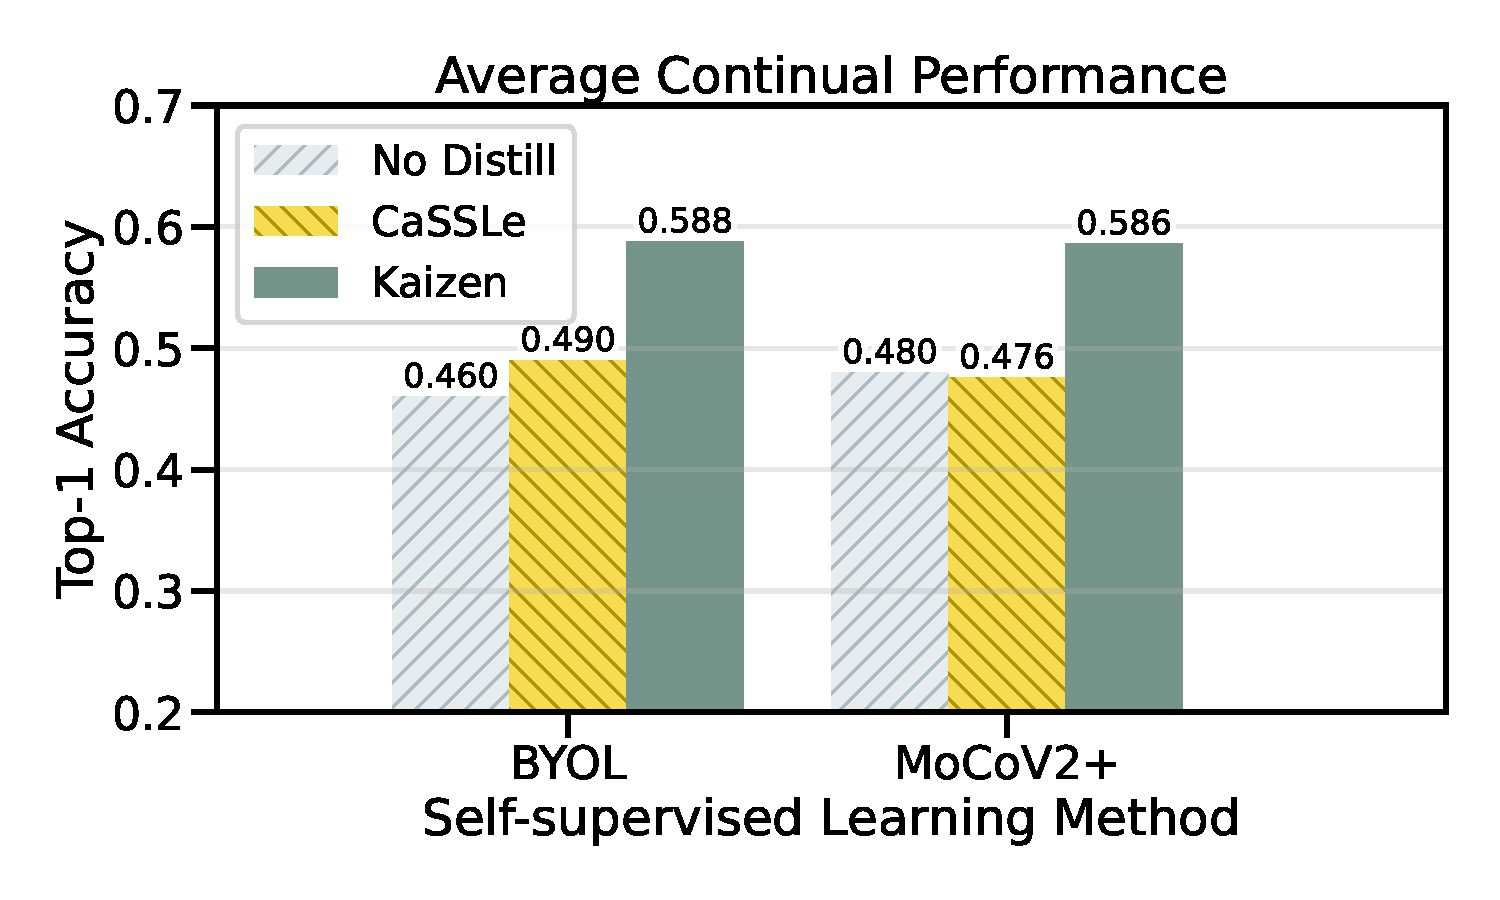
\includegraphics[width=0.7\linewidth]{figures_new/Part_1/F1-WISDM2019-6Tasks-Continual_Accuracy-v2.pdf}\\
   \vspace{-0.1in}
   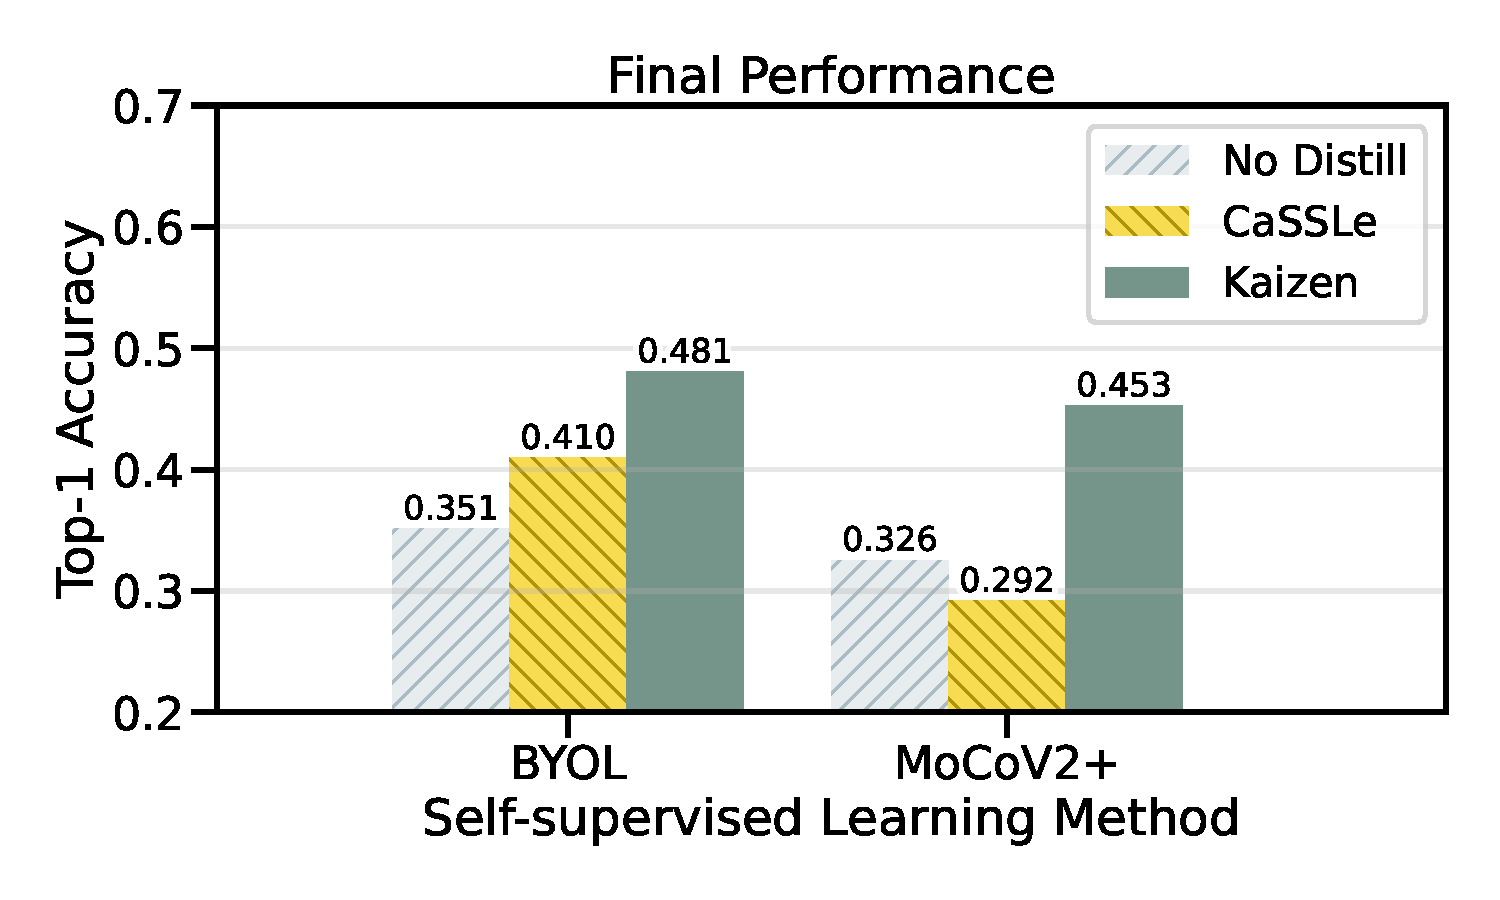
\includegraphics[width=0.7\linewidth]{figures_new/Part_1/F1-WISDM2019-6Tasks-Final_Accuracy-v2.pdf}
   
\end{center}
\vspace{-0.2in}
   \caption{Performance comparison between different training methods. Models are trained using different self-supervised learning methods and knowledge distillation strategies on class-incremental WISDM2019. The top figure shows the average performance across the entire continual learning process, while the bottom figure shows the performance in the final evaluation. 
   }
       \vspace{-0.2in}
   \label{fig:general_performance_comparison}
\end{figure}

To address this data scarcity, continual self-supervised learning (CSSL) leverages self-supervision for continual learning. Recent works \cite{fini2022self, tang2023practical} have demonstrated effectiveness in leveraging different sources of data in continual learning, proposing practical solutions with more practical data assumptions. A discussion about related work can be found in Appx.~\ref{related}.

In this study, we explore CSSL techniques for sensor-based human activity recognition. In particular, we adapted CaSSLe \cite{fini2022self} and Kaizen \cite{tang2023practical} to enable self-supervised and semi-supervised continual learning for activity recognition using accelerometer data. Beyond comparing state-of-the-art methods on comprehensive metrics, we investigated adjusting continual fine-tuning's objective importance. Balancing knowledge retention and new task learning with an adaptive weight corresponding to learned/new class ratios proved most effective for performance across tasks. This work demonstrates realistic continual learning assumptions and balancing objectives to achieve the desired performance for mobile sensing. The results highlight the trade-offs in emphasising knowledge retention or new concepts based on use cases.

% \section{Related Work}
\label{related}
Continual learning has been an active area of research in which many researchers have proposed techniques for mitigating catastrophic forgetting. The main idea behind these methods is to balance stability (retaining knowledge) and plasticity (learning new concepts) for deep learning models. Techniques broadly fall into three categories~\cite{de2021continual}: regularisation-based~\cite{kirkpatrick2017overcoming, li2017learning, shin2017continual, wu2019large}, replay-based~\cite{rebuffi2017icarl, chaudhry2018efficient, ostapenko2019learning, buzzega2020dark}, and parameter-isolation methods~\cite{rusu2016progressive, serra2018overcoming}. State-of-the-art performance often combines these approaches~\cite{mittal2021essentials}.

\subsection{Continual Self-supervised Learning}
However, many existing techniques rely heavily on labelled data, which is often unavailable.  Continual self-supervised learning (CSSL) approaches leverage self-supervised learning to enable continual learning under limited supervision. Initial efforts focused narrowly on self-supervised pre-training combined with supervised continual learning~\cite{gallardo2021self, caccia2022special} or extending contrastive learning frameworks~\cite{cha2021co2l, madaan2021rethinking}. However, these techniques are often designed to work with specific self-supervised learning frameworks. The latest continual self-supervised learning frameworks proposed in existing literature~\cite{de2021continual, fini2022self} have begun investigating more overarching and flexible frameworks, where the model learns continually from a stream of unlabelled data. The work by \cite{tang2023practical} proposed a unified semi-supervised framework with continual fine-tuning, introducing mechanisms for knowledge distillation and new task learning in both representation and classification. These demonstrate progress towards practical solutions under realistic supervision assumptions, and we focus on these recent proposals which repurpose SSL methods for continual learning in this work.

\subsection{Human Activity Recognition}
Wearable-based human activity recognition is an important component in human-centric computing because of its ability to extract real-time information and context clues about user behaviours, which enables other computing applications \cite{choi2016understanding, jaimes2015corredor}. However, the utility of HAR systems has been limited by the scarcity of high-quality labelled data and the computational capabilities of wearable devices.

Since the adoption of deep learning models for HAR, researchers have looked at tackling catastrophic forgetting in HAR specifically \cite{jha2021continual, leite2022resource, schiemer2023online}, and they have demonstrated moderate success. Simultaneously, self-supervised learning has recently gained popularity in the wearable-based HAR community, and many approaches from the general machine learning community, as well as customised methods, have been proposed to leverage unlabelled data to overcome the limitations of labelled data \cite{multi_self_har, tang2020exploring, haresamudram2020masked, tang2021selfhar, haresamudram2021contrastive}. However, we have yet to see efforts in leveraing self-supervised learning techniques for HAR in continual learning. This is an important step towards practical and generalisable user models. CSSL paves the way for realistic solutions to continually learn from combinations of labelled and unlabelled data.

\section{Method}
In this work, we adapted the CaSSLe \cite{fini2022self} and Kaizen \cite{tang2023practical} continual learning frameworks to HAR. This section begins with an overview of these methods and then illustrates the modifications adopted to explore their application to HAR.

\subsection{CaSSLe}
The CaSSLe framework \cite{fini2022self} re-purposed the Siamese/Contrastive learning setup and loss functions for tackling catastrophic forgetting in representation learning. In particular, the framework consists of two main components: new task learning and knowledge distillation.
The \textbf{new task learning (feature extractor)} component follows the conventional Siamese/Contrastive learning setup, like that in BYOL~\cite{grill2020bootstrap} and MoCoV2+~\cite{chen2020improved, he2020momentum}, in which the input signal is transformed into two views using stochastic transformation functions, and the loss function forces the transformed view to have similar representations. The loss term for this is denoted by $\mathcal{L}^{\mathrm{CT}}_{\mathrm{FE}}$.
The \textbf{knowledge distillation (feature extractor)} component mirrors the new task learning component, where the same contrastive loss function is used again, but contrasting the representations retrieved by the feature extractor from the previous task and the current feature extractor instead. An additional predictor (a shallow neural network) is attached to the current feature extractor before contrastive learning. We denote this loss as $\mathcal{L}^{\mathrm{KD}}_{\mathrm{FE}}$.
The CaSSLe framework was shown to be an effective strategy for continual representation learning from a stream of unlabelled data, but it does not propose a specific strategy for training the downstream classifier continually.

\subsection{Kaizen}
The Kaizen framework \cite{tang2023practical} extends CaSSLe by proposing two additional components to handle classifier training, to ensure that a functional classifier is available at any step of the continual learning process.
The \textbf{new task learning (classifier)} component follows conventional supervised learning, in which the classifier is trained using categorical cross-entropy to learn the new classes ($\mathcal{L}^{\mathrm{CT}}_{\mathrm{C}}$).
The \textbf{knowledge distillation (classifier)} component leverages self-distillation to retain knowledge, in which the predictions from the classifier from the previous task are used as pseudo-labels to train the current classifier ($\mathcal{L}^{\mathrm{KD}}_{\mathrm{C}}$). This component does not rely on labelled data and can remain active when only unlabelled data is available.
A small part of the labelled data is retained and replayed, in a similar fashion to other exemplar-based continual learning methods \cite{rebuffi2017icarl, isele2018selective, rolnick2019experience, mittal2021essentials}. This was shown to be a critical component in maintaining classification performance in class-incremental settings \cite{de2021continual}.

\subsection{CSSL for HAR}
\label{subsec:balancing}
As both CaSSLe and Kaizen were proposed for visual representation learning in their original work, we made a few modifications to these frameworks to adapt to HAR.

\subsubsection{Transformation Functions}
Instead of using image transformation functions, we adopted three transformation functions from previous works \cite{har_transformations, multi_self_har, tang2020exploring, tang2021selfhar} that are tailored to sensor time-series: \emph{random 3D rotation}, \emph{random scaling} and \emph{time warping} (see Appx.~\ref{appx:trans}).

\subsubsection{Balancing Learning Objectives}

In addition to following the original formulation of Kaizen, in which the loss function is a sum of all the learning objectives mentioned above 
\[
 \mathcal{L_\mathrm{Kaizen}} =\mathcal{L}^{\mathrm{CT}}_{\mathrm{FE}} + \mathcal{L}^{\mathrm{KD}}_{\mathrm{FE}} + \mathcal{L}^{\mathrm{CT}}_{\mathrm{C}} + \mathcal{L}^{\mathrm{KD}}_{\mathrm{C}}
\]
we hypothesise that the relative importance of the knowledge distillation task compared to learning from new data in classification learning can have a direct impact on the performance of the classifier across time. Therefore, we introduce an importance coefficient $\lambda_{\mathrm{C}}$ to the loss function which allows us to change the weighting of the learning objectives:
\[
 \mathcal{L_\mathrm{Kaizen(adaptive)}} =(\mathcal{L}^{\mathrm{CT}}_{\mathrm{FE}} + \mathcal{L}^{\mathrm{KD}}_{\mathrm{FE}}) + (\mathcal{L}^{\mathrm{CT}}_{\mathrm{C}} + \lambda_{\mathrm{C}} \mathcal{L}^{\mathrm{KD}}_{\mathrm{C}})
\]
The effects of this importance coefficient are explored in our evaluation.

\section{Experimental Setup}
\label{sec:setup}

\paragraph{Data}
We use the Millionbase dataset which is freely available and has close to 2.9 million quality chess games.\footnote{Download link available at \url{https://rebel13.nl/rebel13/rebel\%2013.html}}
After filtering out duplicate games, games with
fewer than 10 moves, and games with
more than 150 moves (for the complete game to fit into one transformer window), we are left with around 2.5 million games.
From this filtered set we randomly select 200K games for training, 15K games each for dev and test, and another 50K games to create board state probing evaluation sets described in Section~\ref{sec:cloze}.
The dev and test sets are used for perplexity evaluations. 
The dev set perplexity is used for choosing hyperparameters.
From the 200K training set, we create subsets of size 15K and 50K which we refer to as ``Train-S'' and ``Train-M'', while the full training set is referred to as ``Train-L''.
For detailed statistics, see Table~\ref{tab:data_stats} in Appendix.
All the data processing steps requiring chess knowledge, including parsing chess databases, are carried out using python-chess~\citep{python-chess}.

To create the board state probing evaluation sets, we use the 50K games reserved for this task. %
We only consider prompts for non-pawn pieces since the dynamics of pawns are fairly limited.
We ensure that the game prefixes selected are never seen in the training data.
The final evaluation set consists of 1000 instances with prefix length (in number of moves) in the range $51 \le l \le 100$.





\begin{figure*}
	\begin{minipage}{\textwidth}
		\begin{minipage}[b]{0.48\textwidth}
			\centering
			\begin{tabular}{llcc}
				\toprule
				Training Set & Model   & Dev set & Test set \\
				\midrule
				\multirow{2}{*}{Train-S} 
				& UCI 				& 23.6 & 23.6\\
				& UCI + RAP 		& 15.9 & 15.9\\
				& UCI + \piecetype 	& 16.1 & 16.2 \\
				\midrule
				\multirow{2}{*}{Train-M} 
				& UCI 				& 11.6 & 11.6\\
				& UCI + RAP 		& 10.4 & 10.4\\
				& UCI + \piecetype 	& 10.1 & 10.0 \\
				\midrule
				\multirow{2}{*}{Train-L} 
				& UCI 				& \phantom{1}7.7 & \phantom{1}7.7\\
				& UCI + RAP 		& \phantom{1}7.4 & \phantom{1}7.4\\
				& UCI + \piecetype 	& \phantom{1}7.2 & \phantom{1}7.2 \\
				\bottomrule
				
			\end{tabular}
			\captionof{table}{Canonical validation and test set perplexity. By canonical we mean that one move, say \pos{f1b5}, counts as one token.}
			\label{tab:perplexity}
		\end{minipage}
		\hfill
		\begin{minipage}[b]{0.48\textwidth}
			\centering
			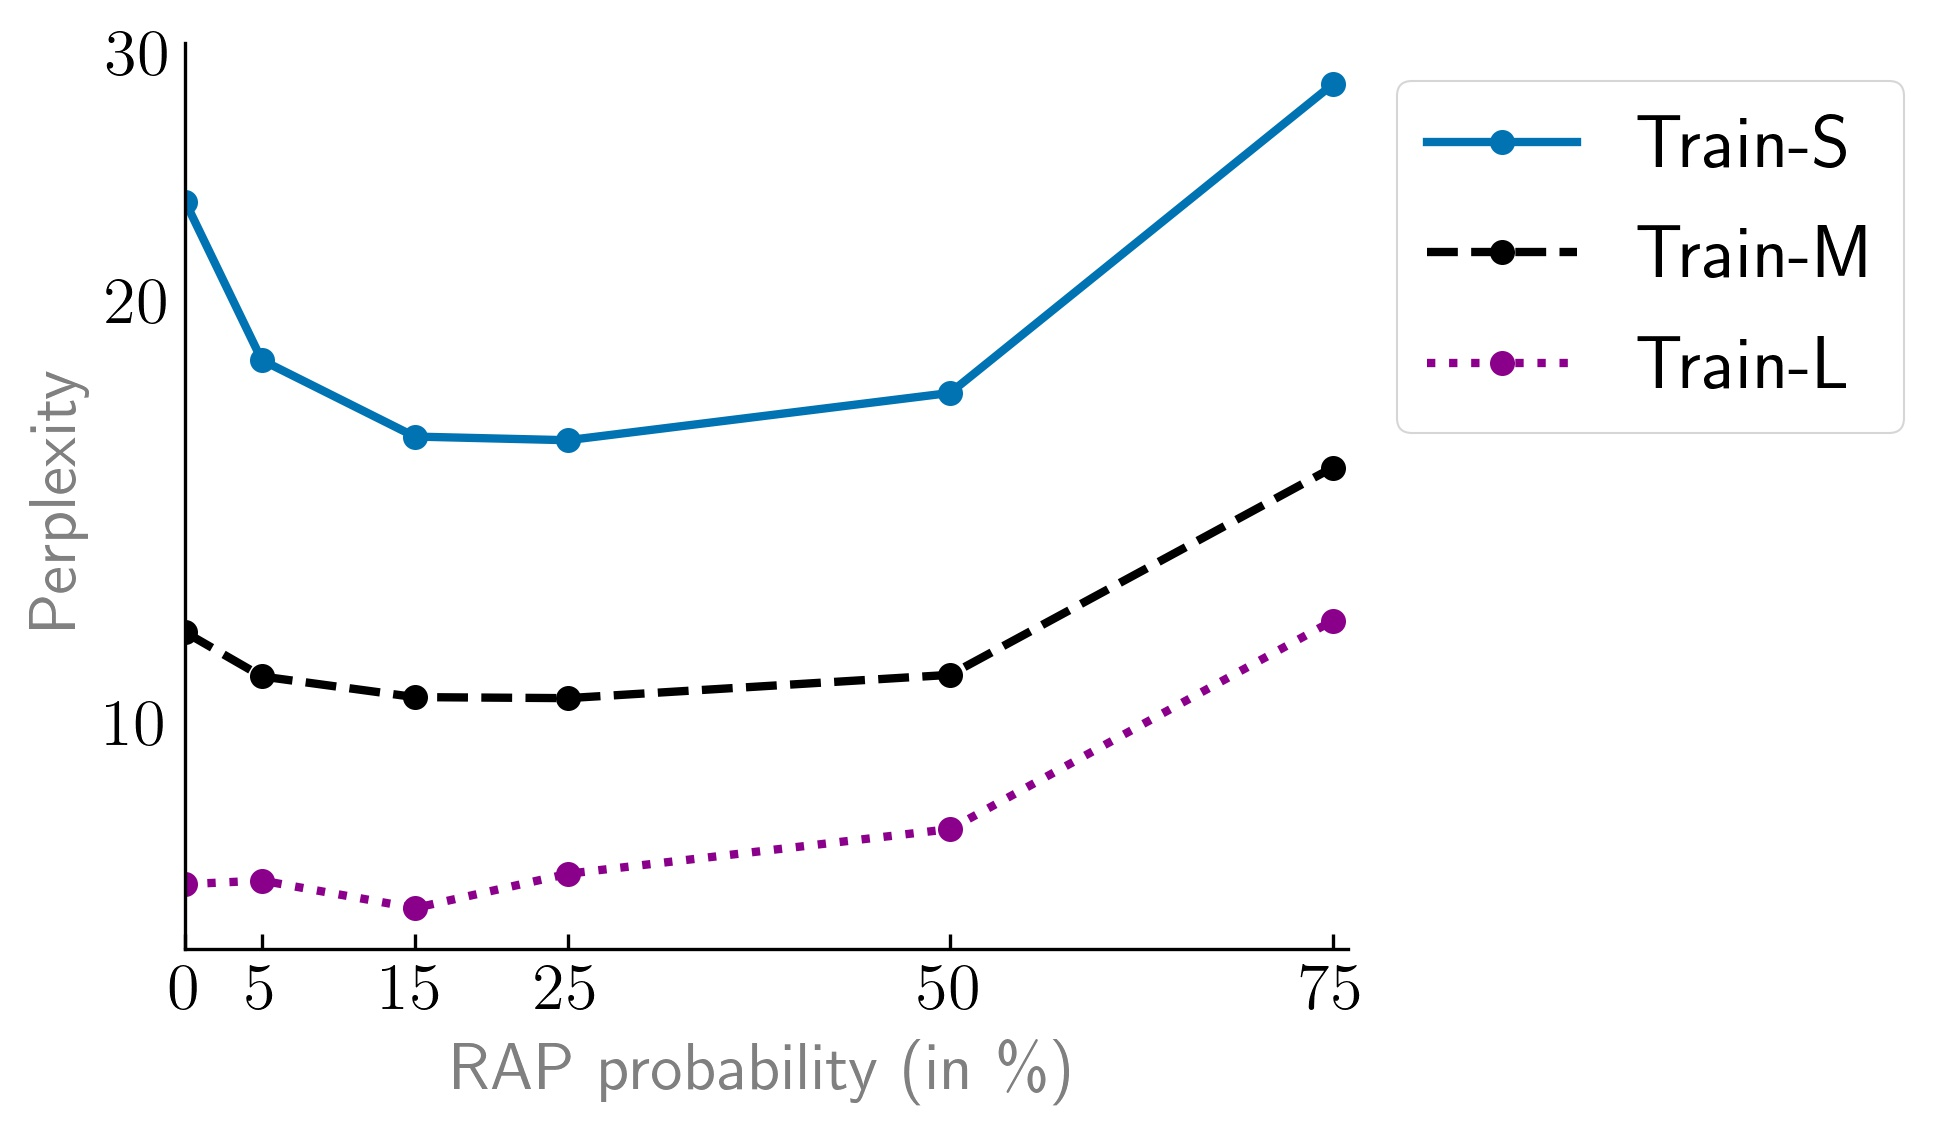
\includegraphics[width=\textwidth]{figures/rap_effect.jpg}
			\captionof{figure}{Validation set perplexities as a function of RAP probabilities for the different training set sizes. RAP $0$ %
				is %
				the standard UCI notation. 
				RAP $100$ is not shown as perplexities are too high. }
			\label{fig:rap_vals}
		\end{minipage}
	\end{minipage}
\end{figure*}

\paragraph{Model Details}
We use the GPT2-small architecture for our base language model \citep{vaswani2017attention,radford2019language}.
GPT2-small is a 12-layer transformer model with 12 attention heads and an embedding size of 768 dimensions.
The context size of the model is limited to 512, which is sufficient to cover the longest game in our training set.
Note that we only borrow the model architecture; the models themselves are \emph{trained from scratch}.
\footnote{Colab notebook to play chess against the base language model \url{https://github.com/shtoshni/learning-chess-blindfolded/blob/master/GPT2_Chess_Model.ipynb}}


For the UCI + RAP $p$ models, we tune over $p \in \{5, 15, 25, 50, 75, 100\}$ based on %
perplexity on the validation set.
Note that for perplexity evaluation, logits corresponding to piece type tokens are masked out since piece type tokens are only available during training.
We find that $p=25$ performs the best for Train-S and Train-M, while $p=15$ is best for Train-L (Figure~\ref{fig:rap_vals}). %
Larger values of $p$ lead to greater mismatch between training and inference, while smaller values likely do not provide enough training signal.

We also experiment with other transformer and non-transformer models in Section~\ref{sec:other_models}.
Among the transformer models, we experiment with two ``approximate" attention models (i.e., models which approximate the full attention of vanilla transformer models), namely, Reformer \cite{kitaev2020reformer} and Performer \cite{choromanski2021rethinking}.  
We set the number of layers and attention heads to 12 for both 
architectures, as in GPT2-small.
We also train LSTM language models with and without RAP. 
For details on hyperparameters and tuning, see Appendix~\ref{sec:hyperparams}.


\paragraph{Training Details}
Models are trained for 10 epochs with a batch size of 60. Validation is performed %
 at the end of every epoch and training stops whenever the validation loss starts increasing.
For optimization we use Adam \citep{kingma2014adam} with learning rate of $5\times10^{-4}$ and L2 weight decay of $0.01$.
The learning rate is warmed up linearly over the first 10\% of training followed by a linear decay.
To accelerate training, we use mixed precision training~\citep{micikevicius2018mixed}. %
All experiments are carried out using the PyTorch Lightning framework %
built on top of PyTorch \citep{falcon2019pytorch, pytorch}.
We use the transformers library \citep{Wolf2019HuggingFacesTS} for all models\footnote{Reformer implementation in \pos{transformers} library is still a work in progress. The presented results are with the 4.2.2 version.} %
except for the Performer model %
for which we use a popular unofficial implementation.
\footnote{\url{https://github.com/lucidrains/performer-pytorch}}









\section{Conclusion}
In this work, we adapted two state-of-the-art CSSL frameworks, CaSSLe and Kaizen, from visual representation learning to human activity recognition, one of the fundamental tasks in human-centric computing. Our evaluation indicates that a unified training scheme handling both representation learning and classification learning, as proposed in Kaizen, can perform better under realistic data assumptions, with the advantage of being deployable at any point during the process, which is particularly vital for HAR and other human-centric applications. Additional experiments indicate that the use of a progressive importance coefficient which adaptively adjusts the importance of knowledge retention and classification learning can allow us to explore the trade-off between different learning objectives, reaching higher levels of performance compared to a fixed loss function. This work demonstrated the potential of utilising self-supervised learning for developing human activity recognition models that can adapt to changes in user behaviours.


\bibliography{aaai24}
\clearpage \newpage
\appendix

\begin{appendix}
    \section{Related Work}
\label{related}
Continual learning has been an active area of research in which many researchers have proposed techniques for mitigating catastrophic forgetting. The main idea behind these methods is to balance stability (retaining knowledge) and plasticity (learning new concepts) for deep learning models. Techniques broadly fall into three categories~\cite{de2021continual}: regularisation-based~\cite{kirkpatrick2017overcoming, li2017learning, shin2017continual, wu2019large}, replay-based~\cite{rebuffi2017icarl, chaudhry2018efficient, ostapenko2019learning, buzzega2020dark}, and parameter-isolation methods~\cite{rusu2016progressive, serra2018overcoming}. State-of-the-art performance often combines these approaches~\cite{mittal2021essentials}.

\subsection{Continual Self-supervised Learning}
However, many existing techniques rely heavily on labelled data, which is often unavailable.  Continual self-supervised learning (CSSL) approaches leverage self-supervised learning to enable continual learning under limited supervision. Initial efforts focused narrowly on self-supervised pre-training combined with supervised continual learning~\cite{gallardo2021self, caccia2022special} or extending contrastive learning frameworks~\cite{cha2021co2l, madaan2021rethinking}. However, these techniques are often designed to work with specific self-supervised learning frameworks. The latest continual self-supervised learning frameworks proposed in existing literature~\cite{de2021continual, fini2022self} have begun investigating more overarching and flexible frameworks, where the model learns continually from a stream of unlabelled data. The work by \cite{tang2023practical} proposed a unified semi-supervised framework with continual fine-tuning, introducing mechanisms for knowledge distillation and new task learning in both representation and classification. These demonstrate progress towards practical solutions under realistic supervision assumptions, and we focus on these recent proposals which repurpose SSL methods for continual learning in this work.

\subsection{Human Activity Recognition}
Wearable-based human activity recognition is an important component in human-centric computing because of its ability to extract real-time information and context clues about user behaviours, which enables other computing applications \cite{choi2016understanding, jaimes2015corredor}. However, the utility of HAR systems has been limited by the scarcity of high-quality labelled data and the computational capabilities of wearable devices.

Since the adoption of deep learning models for HAR, researchers have looked at tackling catastrophic forgetting in HAR specifically \cite{jha2021continual, leite2022resource, schiemer2023online}, and they have demonstrated moderate success. Simultaneously, self-supervised learning has recently gained popularity in the wearable-based HAR community, and many approaches from the general machine learning community, as well as customised methods, have been proposed to leverage unlabelled data to overcome the limitations of labelled data \cite{multi_self_har, tang2020exploring, haresamudram2020masked, tang2021selfhar, haresamudram2021contrastive}. However, we have yet to see efforts in leveraing self-supervised learning techniques for HAR in continual learning. This is an important step towards practical and generalisable user models. CSSL paves the way for realistic solutions to continually learn from combinations of labelled and unlabelled data.

\section{Transformation Functions}
\label{appx:trans}

\noindent\textbf{Random 3D rotation} applies a random rotation in the 3D space by picking a random axis in 3D and a rotational angle from uniform distributions. This is to simulate common pose changes in wearable devices.

\noindent\textbf{Random scaling} alters the size of samples within a window by multiplying them with a randomly chosen scalar. We apply this transformation since a model that can handle these scaled signals creates better representations because it learns to be unaffected by changes in amplitude and offset.

\noindent\textbf{Time warping} locally stretches or warps the time series data, smoothly distorting the time intervals between sensor readings.
\section{Evaluation setup}
\label{appx:setup}
{
\subsection{Model Architecture}
In this work, we adopted a lightweight HAR model, TPN \cite{multi_self_har}, to replace the vision-based model.

\subsection{Evaluation Metrics}
For the evaluation metrics, we are adopting the same framework as introduced in Kaizen \cite{tang2023practical}: \textbf{Final Accuracy (FA)}, \textbf{Continual Accuracy (CA)}, \textbf{Forgetting (F)}, and \textbf{Forward Transfer (FT)} as metrics. This set of values can better reflect the performance of continual learning methods in different use cases.

\subsection{Self-supervised Learning Frameworks}
In this work we selected a contrastive-based method MoCoV2+~\cite{chen2020improved, he2020momentum}, and an asymmetric-model-based method
BYOL~\cite{grill2020bootstrap} as the self-supervised learning method for continual learning. These two methods have been shown to be well-performing in continual self-supervised learning settings~\cite{fini2022self, tang2023practical}, and our goal is to investigate whether different CSSL methods demonstrate different performance characteristics when using different SSL methods as the knowledge retention mechanism.

\subsection{Dataset}
We performed our evaluation using the WISDM2019 (WISDM Smartphone and Smartwatch Activity and Biometrics Dataset) \cite{weiss2019wisdm}, which is an activity recognition dataset collected by the WISDM (Wireless Sensor Data Mining) Lab in the Department of Computer and Information Science of Fordham Unversity. The dataset contains raw accelerometer and gyroscope data from a smartwatch (LG G Watch) and a smartphone (Google Nexus 5/5x or Samsung Galaxy S5) worn by 51 subjects, who performed 18 different activities for 3 minutes each. The smartphone is placed inside the participant's pocket, while the smartwatch is worn at the dominant hand. The data was collected at a sampling rate of 20Hz for the following activities: Walking, Jogging, Stairs, Sitting, Standing, Typing, Brushing Teeth, Eating Soup, Eating Chips, Eating Pasta, Drinking from Cup, Eating Sandwich, Kicking (Soccer Ball), Playing Catch with Tennis Ball, Dribbling (Basketball), Writing, Clapping, and Folding Clothes. The accelerometer data from the smartwatch was used in this study, and we selected this dataset for evaluation because it has a relatively high number of activities in HAR, which makes it suitable for continual learning evaluation.

The raw sensor data underwent minimal pre-processing. First, z-normalization was applied using the training data's mean and standard deviation for each sensor channel. Next, the data was segmented into \(384 \times 3\) sliding windows, representing 384 timestamps and 3 triaxial accelerometer channels. Consecutive windows do not overlap. 20-25\% of user data was held out unseen as the test set to evaluate model generalisability. 

The 18 classes of activities are randomly and evenly split into 6 tasks of 3 classes each with no overlap as follows: task 1 - \{Folding Clothes, Stairs, Walking\}, 
task 2 - \{Sitting, Drinking from Cup, Eating Chips\}, 
task 3 - \{Standing, Eating Sandwich, Clapping\}, 
task 4 - \{Brushing Teeth, Jogging, Eating Pasta\},
task 5 - \{Eating Soup, writing, Typing\}, and
task 6 - \{Playing Catch with Tennis Ball, Kicking (Soccer Ball), Dribbling (Basketball)\}. This follows the conventional setup of class-incremental learning, and how different (potentially qualitative) splitting of the classes affects model performance is left as future work.

\subsection{Baselines}
\label{subsection:baselines}
We followed the evaluation setup as proposed in \cite{tang2023practical}, in which we compare the performance of Kaizen, CaSSLe, as well as a \emph{No distill} baseline that fine-tunes the full model on new tasks with no explicit catastrophic forgetting mitigation. As CaSSLe and \emph{No distill} baselines are self-supervised learning methods without incorporating a classifier, the classifiers are trained separately after the feature extractor is trained, with data replay enabled.
}
\end{appendix}

\section{Additional Visualisations}
\label{subsection:additional_results}
\begin{figure}
    \centering
    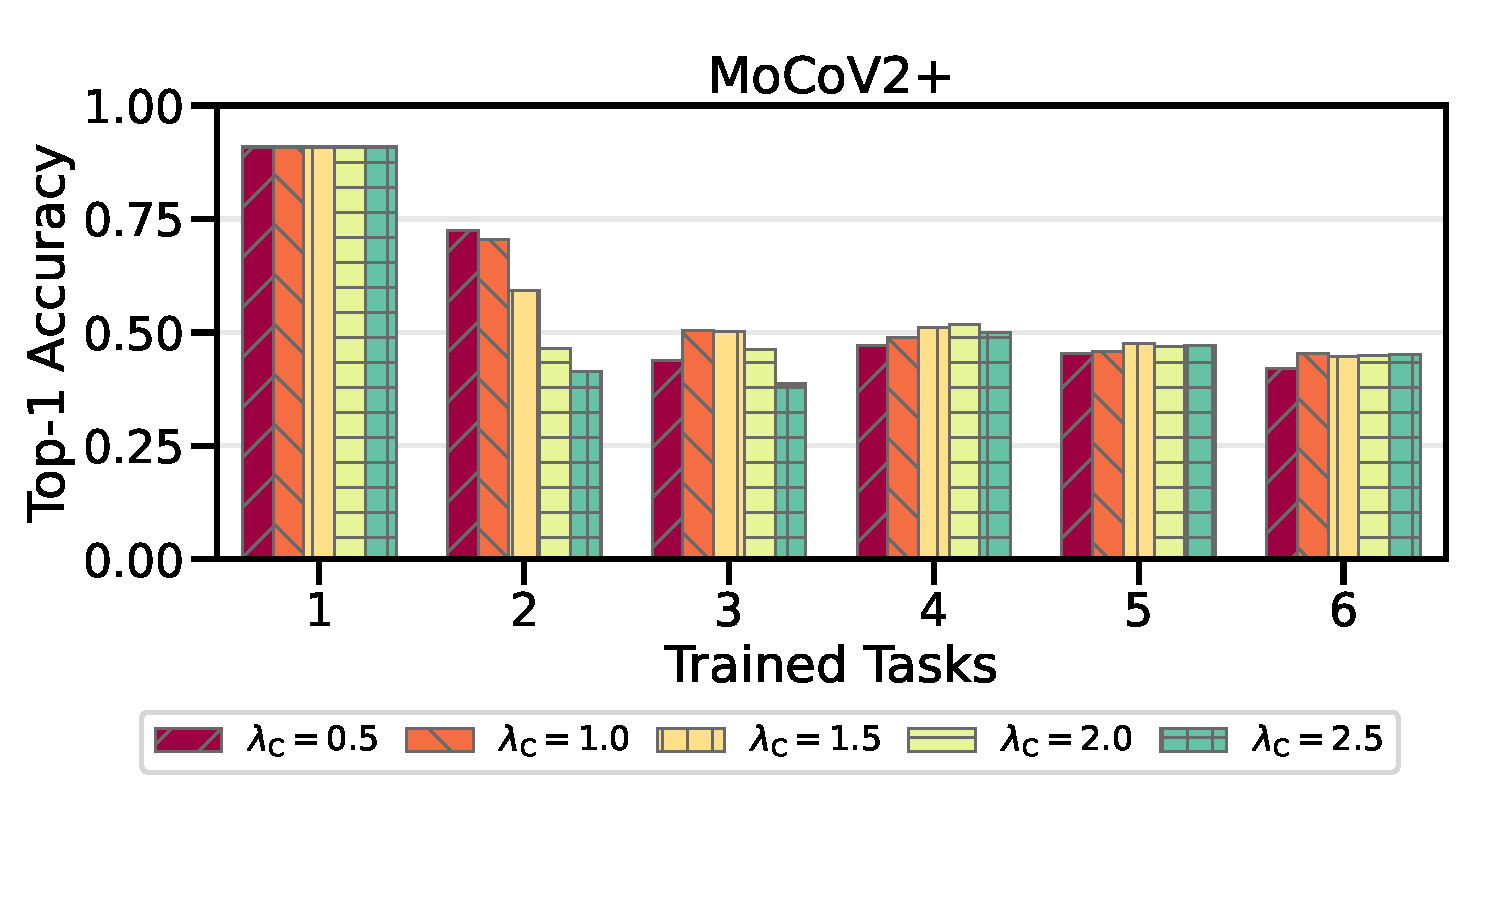
\includegraphics[width=0.8 \linewidth ]{figures_new/Part_2/F3-WISDM2019-MoCoV2+-6Tasks-v2.pdf}
    % \vspace{-0.3in}
    \caption{Performance after training on different tasks with varying constant importance coefficients.}
\label{fig:kaizen_performance_across_time_constant_lamb}
\end{figure}


\begin{figure}
    \centering
    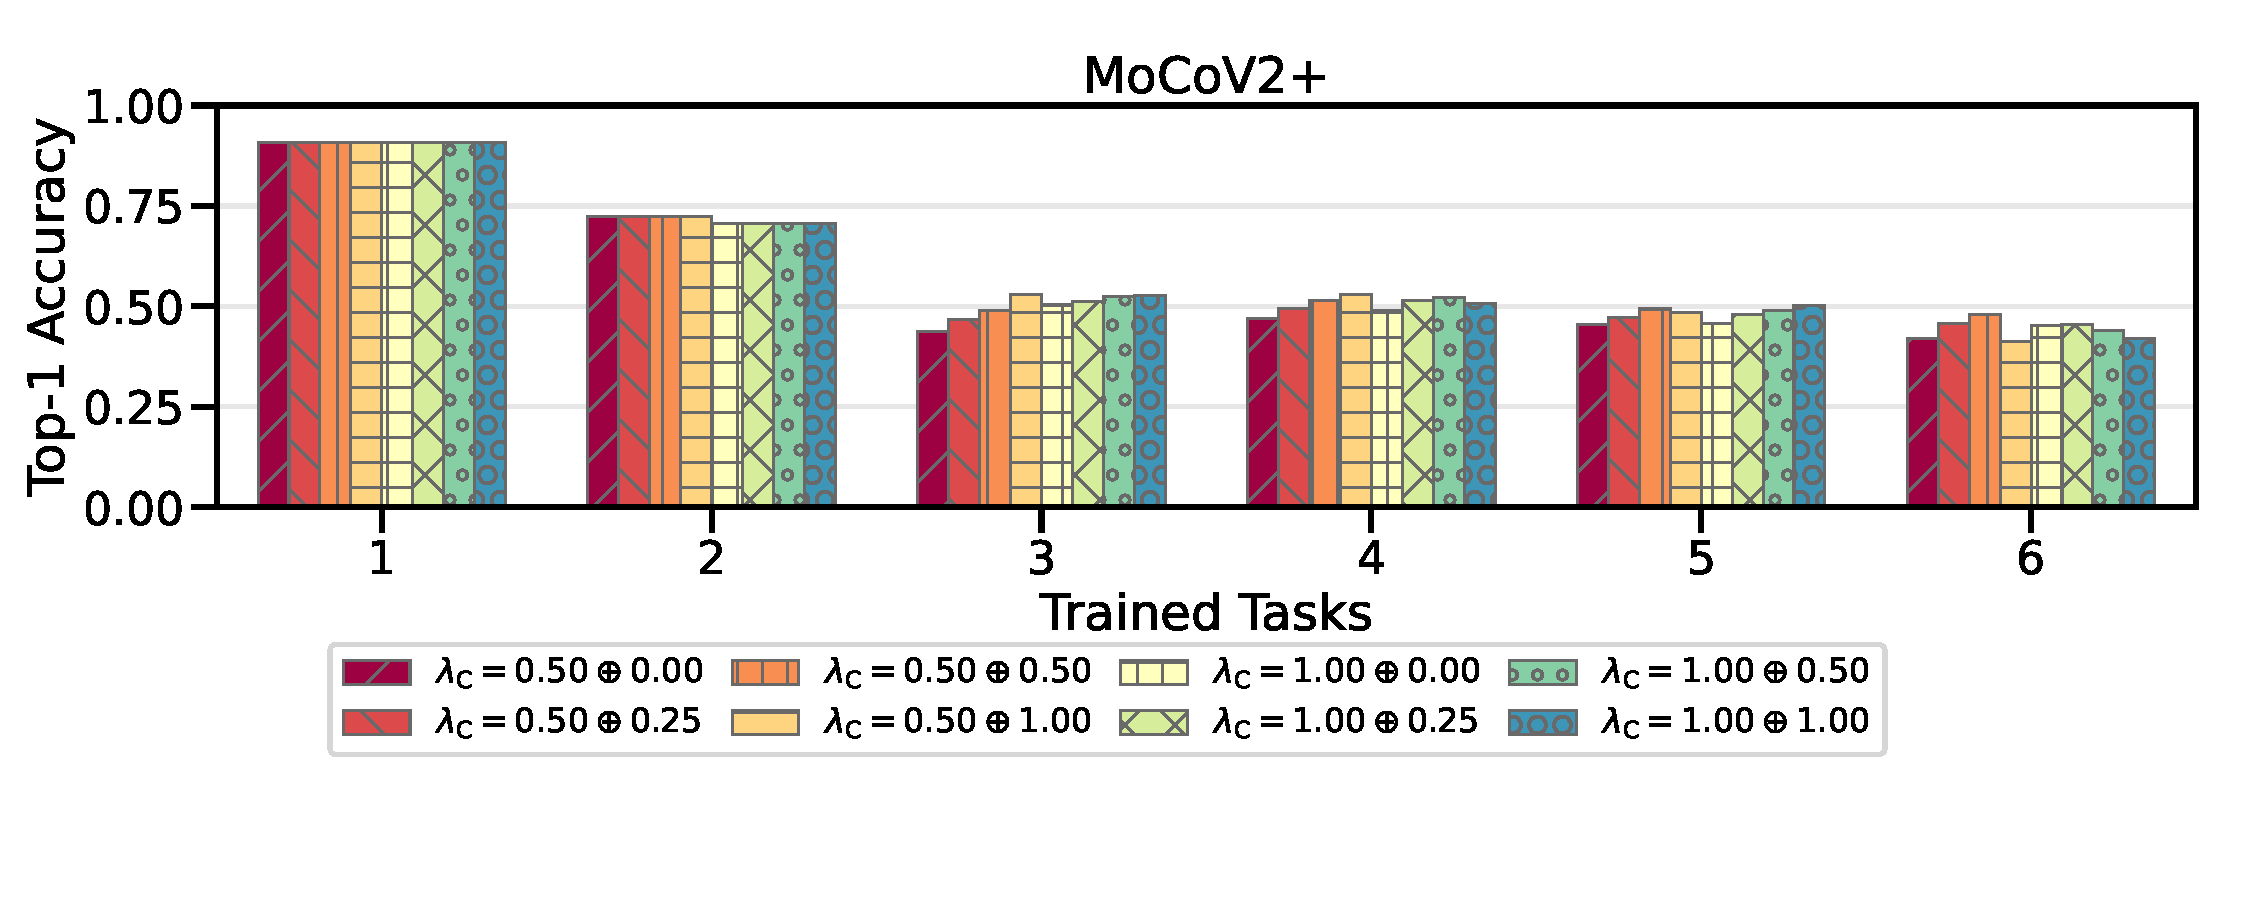
\includegraphics[width=0.99 \linewidth ]{figures_new/Part_3/F3-WISDM2019-MoCoV2+-6Tasks-v2.pdf}
    % \vspace{-0.3in}
    \caption{Performance after training on different tasks with varying progressive importance coefficients.}
\label{fig:kaizen_performance_across_time_progressive_lamb}
\end{figure}

Fig.~\ref{fig:kaizen_performance_across_time_constant_lamb} and \ref{fig:kaizen_performance_across_time_progressive_lamb} illustrate the aggregated performance of models trained with Kaizen after each task with different importance coefficients.

\end{document}
